\chapter{Nutzerstudie}
\label{chap:evaluation}
Aus \autoref{chap:related_work} geht hervor, dass der Abgleich von 2D-Karten mit der Umgebung einen gewissen mentalen Aufwand erfordert, bedingt durch das Fehlen einer Dimension.
Die 2D-Karte ist eine Abstraktion der Umgebung, wodurch Informationen verloren gehen.
Der Zweck dieser Nutzerstudie ist zu überprüfen, ob sich bei den Probanden durch die 3D-Megamap ein räumliches Verständnis aufbaut, welches gegenüber der 2D-Karte zu einer effektiveren und effizienteren Orientierung führt.
Um dies zu testen führen die Probanden eine Suchaufgabe und eine Richtungseinschätzung durch.
Dabei werden unter anderem die Suchzeit, die Abweichung der Schätzung und die Trefferrate des Ziels zwischen den Kartenvarianten verglichen.
Außerdem bewerten die Probanden die Nutzbarkeit der Ansätze und geben Feedback zum Megamap-Prototypen.

Die Hypothesen, die mit dieser Studie getestet werden, sind wie folgt definiert:
\begin{itemize}
    \item Nullhypothese ($H_0$): Es gibt keine messbaren Unterschiede zwischen der 2D-Karte und den Megamaps bezüglich Effektivität und Effizienz.
    \item $H_a$: Die Effektivität und Effizienz der Megamaps unterscheiden sich von der 2D-Karte.
\end{itemize}

\section{Aufbau}
Das Experiment wurde im Laborraum 5220 (MZH Ebene 5) der Arbeitsgruppe Human-Computer Interaction an der Universität Bremen durchgeführt.
Für die Präsentation der virtuellen Umgebung wurde die HTC Vive mit zwei Basisstationen eingesetzt.
Der getrackte Bereich zwischen den Basisstationen umfasste ca. \SI{3}{\metre} $\times$ \SI{3}{\metre}.
Die Bilddaten wurden von einem PC mit einer \emph{Nvidia~GTX~1080~Ti} Grafikkarte und einem \emph{AMD~Ryzen~7~1800X} Prozessor mit Unity~2018.2.12f1 gerendert.
Übertragen wurden die Bilddaten an das HMD mit dem \emph{VIVE~Wireless~Adapter} \parencite{HTCCorporation2018b}.
Die Fragebögen wurden über \emph{Google Forms} erstellt und ausgefüllt.
Hierfür wurde ein separater Laptop bereitgestellt.

\section{Konditionen und Aufgaben}
\label{sec:conditions_and_tasks}
Die Studie wurde als Experiment innerhalb einer Gruppe (\emph{Within-Subject}) gestaltet.
Für die Nutzerstudie wurden drei unterschiedliche Konditionen getestet (siehe \autoref{fig:conditions}):
\begin{itemize}
    \item $3D_l$ (\emph{low)}: Die 3D-Megamap wird mit einer Skalierung von \SI{6}{\percent} (relativ zur Umgebung) und \SI{25}{\cm} über dem Boden angezeigt.
    Diese Kondition entspricht am ehesten der Megamap aus TCTD. 
    \item $3D_h$ (\emph{high}): Die 3D-Megamap wird mit einer Skalierung von \SI{6}{\percent} (relativ zur Umgebung) und \SI{1}{\metre} unterhalb der HMD-Position angezeigt.
    Dabei wird die Höhe nur beim Aufrufen der Karte berechnet.
    Danach bleibt sie fix.
    Diese Kondition wird getestet, um zu ermitteln, wie sich die Höhe der Megamap vom Boden auf die Nutzung auswirkt (insbesondere unter dem Aspekt, dass durch die Darstellung in 3D Verdeckungen durch die Wände der Räume auftreten können).
    \item $2D$: Eine 2D-Karte wird senkrecht an der Wand vor dem Nutzer angezeigt.
    Auch die 2D-Karte hat eine Skalierung von \SI{6}{\percent} (relativ zur Umgebung).
    Die Karte ist so an der Wand platziert, dass sie weder von anderen Wänden, noch von der Decke oder dem Fußboden geschnitten wird.
\end{itemize}
\begin{figure}[h]
    \begin{subfigure}{0.33\linewidth}
        \centering
        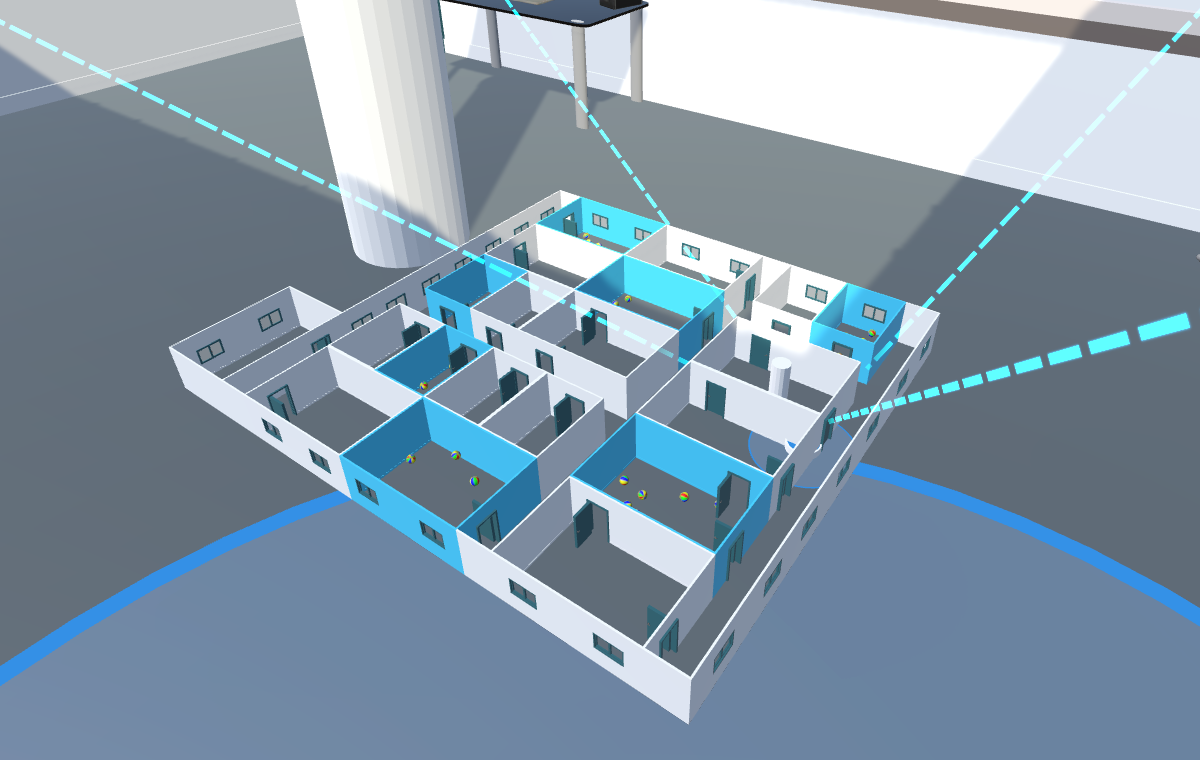
\includegraphics[width=\linewidth]{figures/screenshots/condition_3d_l_x}
        \caption{$3D_l$}
    \end{subfigure}%
    \hfill
    \begin{subfigure}{0.33\linewidth}
        \centering
        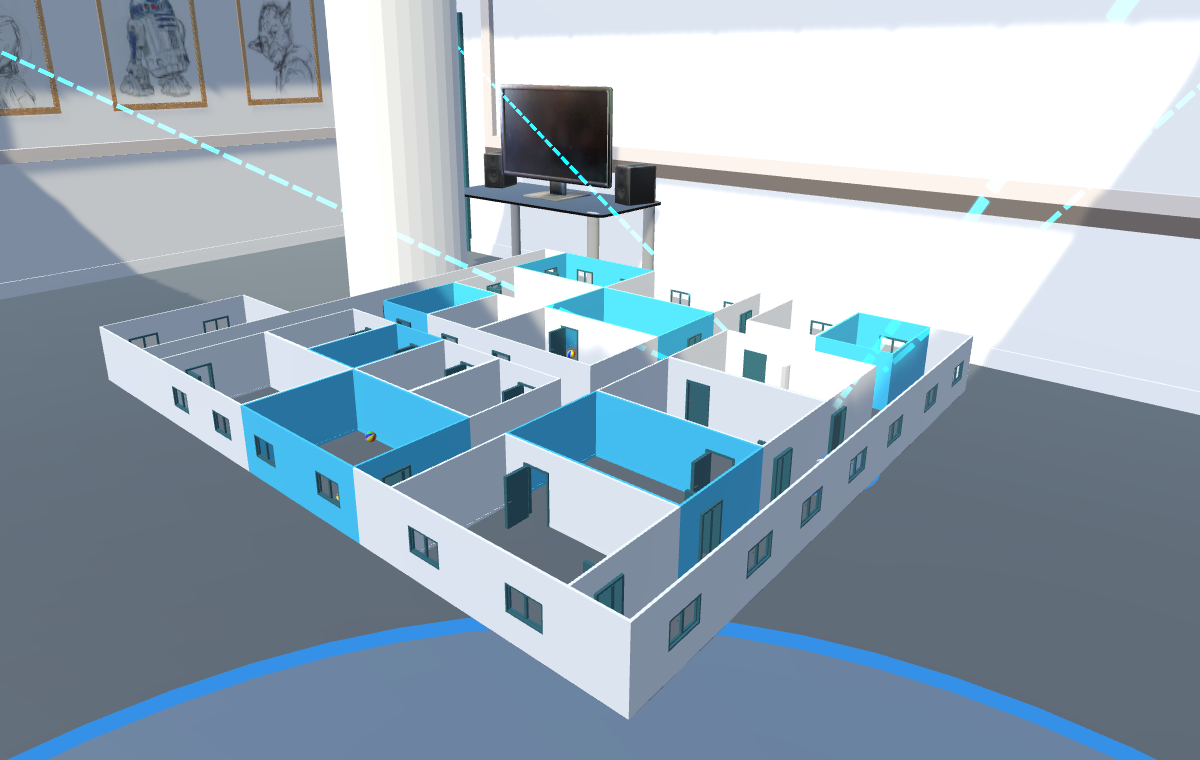
\includegraphics[width=\linewidth]{figures/screenshots/condition_3d_h_x}
        \caption{$3D_h$}
    \end{subfigure}%\\
    \hfill
    \begin{subfigure}{0.33\linewidth}
        \centering
        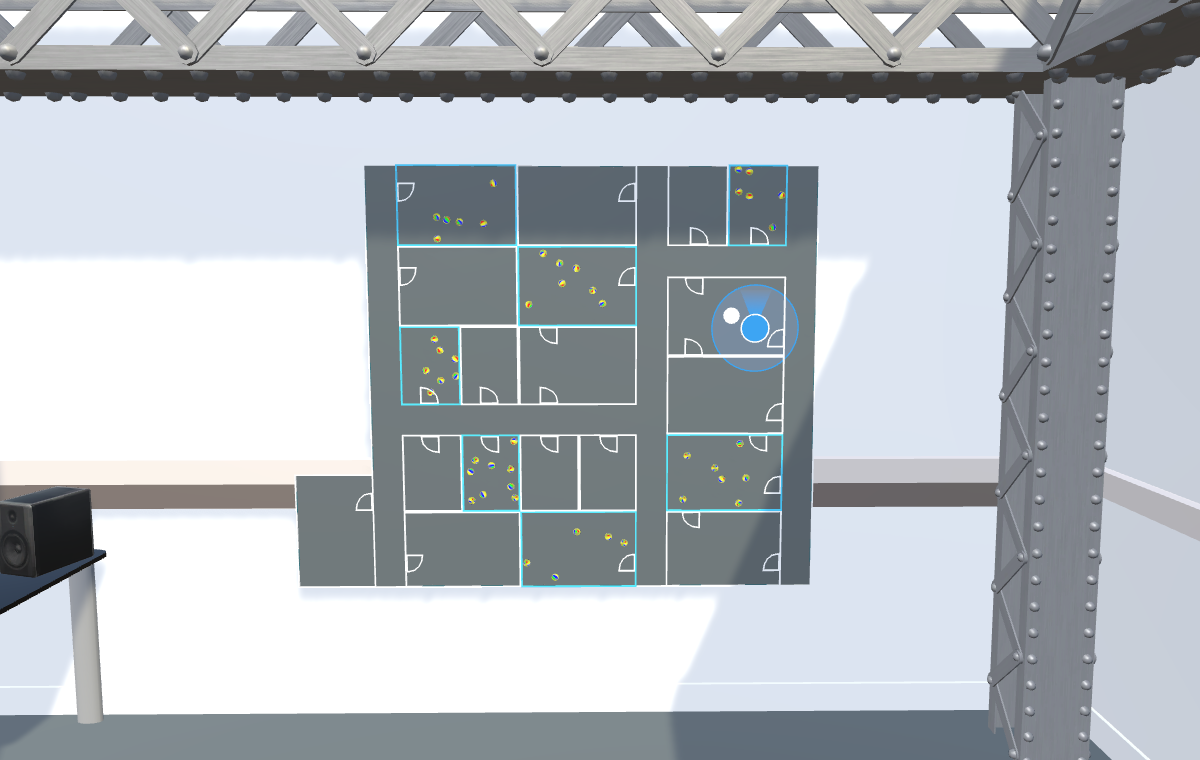
\includegraphics[width=\linewidth]{figures/screenshots/condition_2d_x}
        \caption{$2D$}
    \end{subfigure}%
    \caption{Die drei getesteten Konditionen.}
    \label{fig:conditions}
\end{figure}
Jedem Proband wurde vor dem Experiment eine von sechs möglichen Abfolgen der Konditionen zugeordnet.
Den Probanden wurde ihre jeweilige Sequenz nicht mitgeteilt.
Die Verteilung der Probanden auf die Sequenzen befindet sich im Anhang in \autoref{appendix:condition_sequences}.
Da 15~Probanden teilgenommen haben sind die Sequenzen ungleichmäßig verteilt.

Jede Kondition wurde über 6~Iterationen wiederholt.
Dabei wurde in jeder Iteration eine andere Indoor-Karte für die Megamap verwendet, um einen Lerneffekt der Kartenlayouts zu minimieren.
Die unterschiedlichen Karten sind in \autoref{fig:maps} zu sehen.
Damit die Konditionen vergleichbar bleiben, wurde jede Karte einmal jeder Kondition unterzogen.
Das heißt, die Probanden durchliefen insgesamt 18~Iterationen, wobei sechs unterschiedliche Karten jeweils dreimal eingesetzt wurden.
Die Reihenfolge der Iterationen innerhalb einer Kondition war zufällig bestimmt, wobei darauf geachtet wurde, dass bei einem Wechsel der Konditionen die gleiche Karte nicht zweimal aufeinander folgte.
\begin{figure}[h]
    \centering
    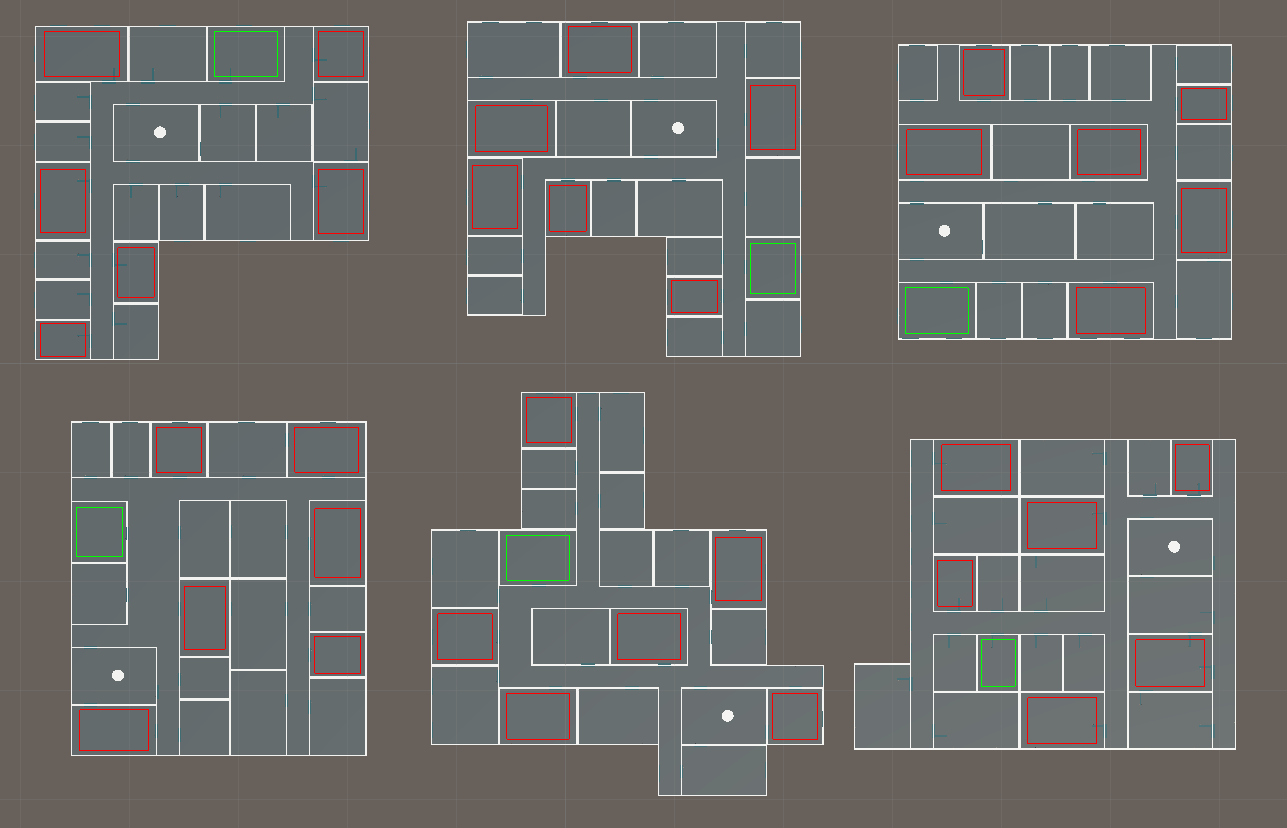
\includegraphics[width=\linewidth]{figures/screenshots/maps_all}
    \caption{Die sechs verwendeten Kartenlayouts. %
    Alle \textcolor{red}{rot} markierte Räume werden mit Bällen gefüllt. %
    Der Zielraum ist \textcolor{green}{grün} markiert. %
    Der Laborraum ist der Raum mit der Säule (weißer Punkt).}
    \label{fig:maps}
\end{figure}

Um die Auswirkungen der jeweiligen Kondition auf die Performance und die räumliche Wahrnehmung des Probanden zu testen, wurden eine Suchaufgabe und eine Richtungsschätzung in den Megamap-Prototypen integriert.

Für die Suchaufgabe wurden auf der jeweiligen Karte in sieben Räumen Bälle platziert (rote Räume in \autoref{fig:maps} und Zielraum).
Die Probanden mussten dann den Raum suchen, der die meisten Bälle enthielt und diesen mit dem Vive~Controller und dem virtuellen Laserpointer auswählen.
Jede Megamap hatte genau einen Zielraum, welcher zufällig zwischen sieben und zehn Bällen enthielt.
Die anderen Räume enthielten mindestens fünf Bälle und maximal einen Ball weniger, als der Zielraum.
Jede der sechs Indoor-Karten hatte denselben Zielraum in allen drei Konditionen.
So bleiben die Karten über die Konditionen hinweg vergleichbar.
Wäre immer ein anderer Zielraum gewählt worden, wäre der Schwierigkeitsgrad der Suche zwischen den Konditionen bei gleicher Karte verschieden gewesen.
Für den Fall, dass ein Proband einen falschen Raum auswählte, wurde dieser rot eingefärbt.
Der Proband musste dann mit der Suche nach dem Zielraum fortfahren.

Anhand der Megamap mussten sich die Probanden die Richtung vom virtuellen Laborraum zum Zielraum (horizontal und vertikal zentriert) merken.
Sobald sie den Zielraum ausgewählt hatten, wurde die Megamap ausgeblendet.
Mit dem virtuellen Laserpointer sollten die Probanden dann möglichst mittig auf den Zielraum \emph{in ihrer Umgebung} zeigen.
Durch Betätigen des Triggers konnte der Laserpointer \enquote{eingefroren} werden, um die Richtung entweder zu korrigieren oder zu akzeptieren.
Wenn die Richtung akzeptiert wurde, startete die nächste Iteration.

Damit die Suche auf einer Karte über alle Konditionen hinweg von der gleichen Position startete, wurde ein \emph{User Setup} implementiert.
Die beiden Schritte des User Setups sind in \autoref{fig:user_setup} zu sehen.
Die Probanden mussten sich auf eine festgelegte Zielposition stellen und für zwei Sekunden auf ein Ziel an der Wand schauen.
Die beiden Zielpositionen waren von der jeweiligen Karte abhängig, blieben jedoch für eine Karte über die Konditionen hinweg gleich.
Für jede Karte galten somit in allen Konditionen die gleichen Ausgangsbedingungen.
Das User Setup wurde ebenso zwischen vor der Richtungsschätzung implementiert.
Ohne diesen Zwischenschritt hätten die Probanden in den 3D-Konditionen nur den Laserpointer vom Raum auf der Karte anheben müssen, um die korrekte Richtung zu schätzen.
Durch das User Setup wurden die Probanden abgelenkt, was diesen Vorteil der 3D-Konditionen gegenüber der 2D-Kondition minimieren sollte.
\begin{figure}[h]
    \begin{subfigure}{0.49\linewidth}
        \centering
        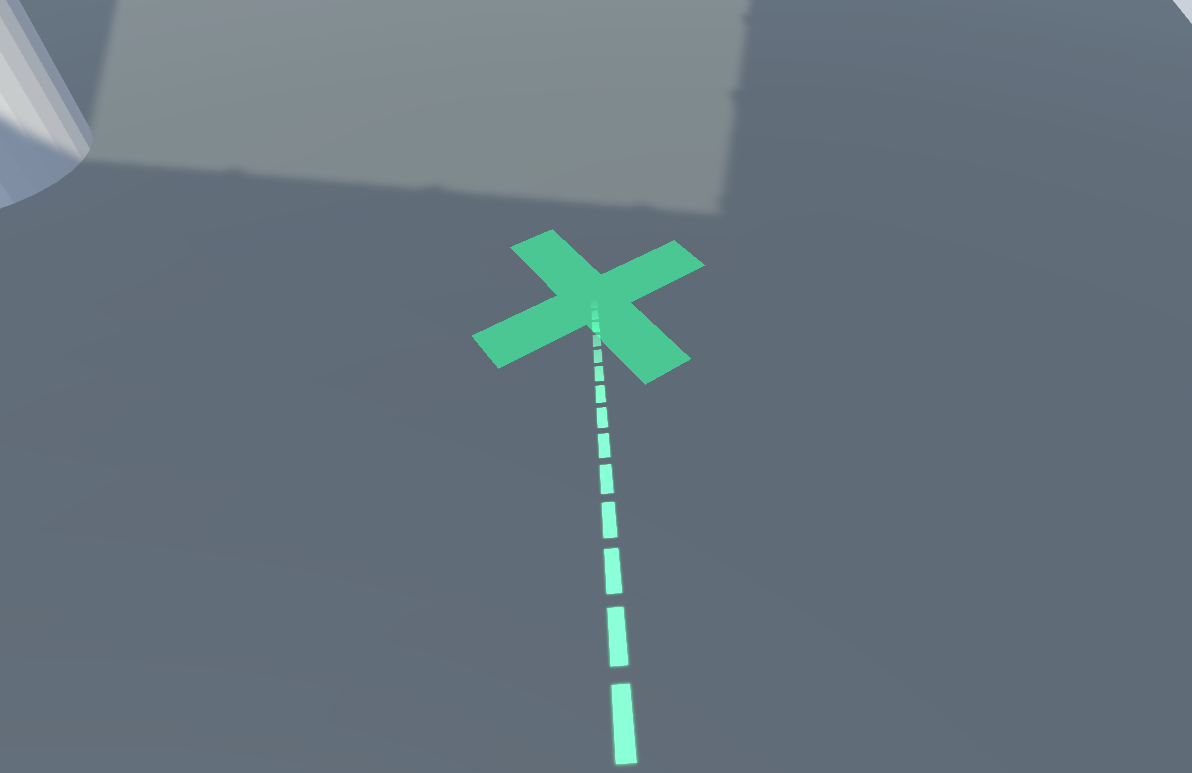
\includegraphics[width=\linewidth, height=5cm]{figures/screenshots/user_setup_floor}
        \caption{}
        \label{sfig:user_setup_floor}
    \end{subfigure}%
    \hfill
    \begin{subfigure}{0.49\linewidth}
        \centering
        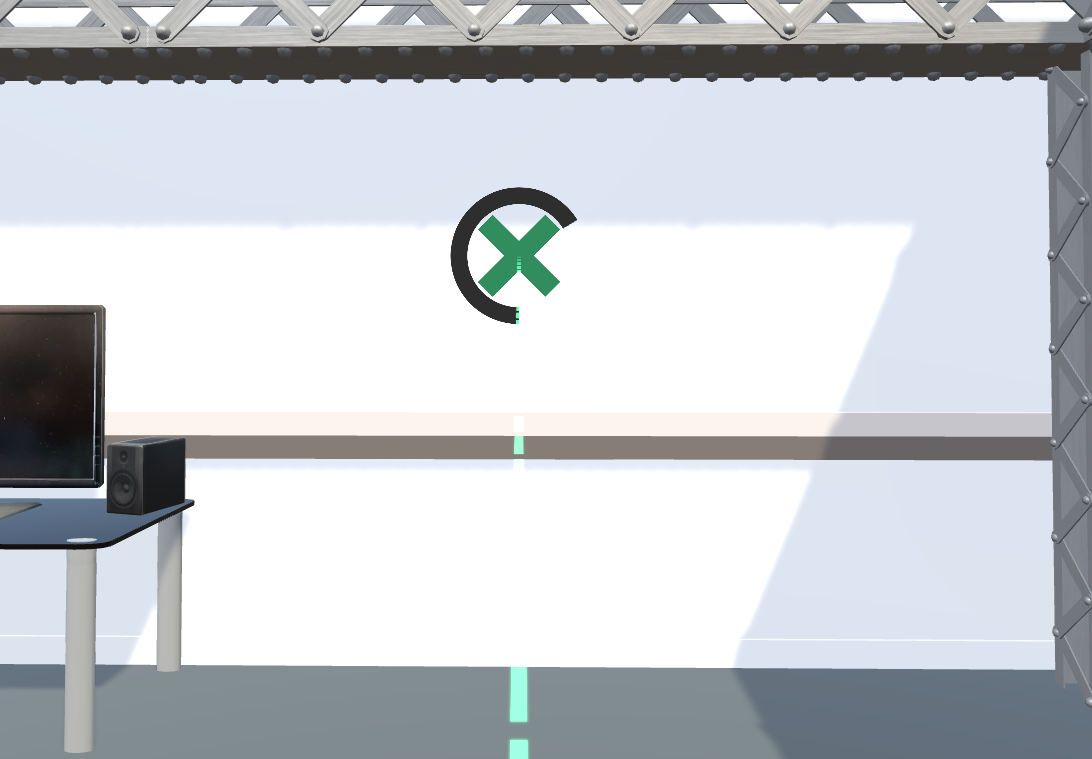
\includegraphics[width=\linewidth]{figures/screenshots/user_setup_wall}
        \caption{}
        \label{sfig:user_setup_wall}
    \end{subfigure}
    \caption{Mit dem \enquote{User Setup} wurde vor der Raumsuche die Startposition und Blickrichtung zwischen den Konditionen angeglichen. %
    Vor der Schätzung der Richtung wurden die Probanden außerdem abgelenkt. %
    \textbf{(\subref{sfig:user_setup_floor})} Die Probanden mussten sich zuerst auf das 'X' stellen. %
    \textbf{(\subref{sfig:user_setup_wall})} Danach mussten die Probanden für \SI{2}{\second} auf das Ziel an der Wand schauen.}
    \label{fig:user_setup}
\end{figure}

\section{Ablauf}
Für einen Test wurden \num{45}~Minuten angesetzt.
Zuerst bekamen die Probanden Hintergrundinformationen zu der Nutzerstudie (siehe Anhang \autoref{appendix:study_infos}).
Unter anderem wurde erklärt, dass eine neuartige 3D-Darstellung von Indoor-Karten für MR/VR getestet wird und dass 2D- und 3D-Varianten verglichen werden.
Mit einem Informationsbogen wurden die Probanden über die Details, den Ablauf sowie die gesammelten Daten der Nutzerstudie aufgeklärt.
Daraufhin unterschrieben die Probanden einen Zustimmungsbogen (siehe Anhang \autoref{appendix:study_consent}).
Damit willigten sie zur Teilnahme an der Studie sowie der Aufzeichnung ihres Blickfelds in der virtuellen Umgebung ein.
Die Probanden konnten frei entscheiden, ob zusätzlich eine Audioaufnahme der Gespräche während des Experiments aufgezeichnet wird.
 
Vor dem eigentlichen Test füllten die Probanden einen demografischen Fragebogen aus (siehe Anhang \autoref{appendix:demographic}).
Dieser enthielt Fragen zur Person (Alter, Geschlecht usw.) sowie Vorerfahrungen in VR/MR und mit Kartenanwendungen für Außen- und Innenbereiche. Der letzte Teil des Fragebogens enthielt die ins Deutsche übersetzte Santa~Barbara~Sense-of-Direction~Skala (SBSOD) \parencite{Hegarty2002}, durch den die Probanden eine Selbstauskunft über ihren Orientierungssinn gaben.
Die Bewertung wurde von einer 7-Punkte- auf eine 5-Punkte-Likert-Skala abgeändert, um mit den anderen Fragebögen einheitlich zu sein.

Den Probanden wurde danach das VR-Equipment (HMD und Batteriepack für den Wireless~Adapter) angelegt.
Sie fanden sich im virtuellen Laborraum wieder.
Die Probanden wurden kurz in der Bedienung des Vive~Controllers und der Bewegung im Raum innerhalb der Play Area unterrichtet.
Sie wurden darauf hingewiesen, dass an einer der Wände ein virtueller Bildschirm hing, der ihnen den nächsten Aufgabenschritt in Textform anzeige, sollten sie den Ablauf vergessen haben.
Die Probanden konnten darüber hinaus jederzeit während des Experiments Fragen an den Versuchsleiter stellen.

Es folgte ein Tutorial, bei dem die Probanden die zuvor beschriebenen Aufgaben (User~Setup --- Suche --- User~Setup --- Schätzen) in einer Tutorialkondition durchliefen (\SI{40}{\cm} Kartenhöhe vom Boden bei \SI{4}{\percent} Skalierung).
Zuerst wurde die 3D-Megamap gezeigt, danach die 2D-Kondition.
Die Probanden konnten entscheiden, ob sie das Tutorial wiederholen oder fortfahren wollen.

Nach dem Tutorial durchliefen die Probanden die Konditionen und Aufgaben, wie sie in \autoref{sec:conditions_and_tasks} beschrieben sind.
Zwischen den Kondition setzten die Probanden das HMD ab und füllten am Laptop einen Fragebogen zur zuletzt getesteten Kartenvariante aus (siehe \autoref{appendix:sus}).
Die Fragebögen basierten auf der \emph{System~Usability~Scale} (SUS) \autocite{Brooke2013}, wurden jedoch für das Anwendungsgebiet von Karten angepasst.
Die Bewertung der einzelnen Aussagen erfolgte über eine 5-Punkte-Likert-Skala.

Nach Abschluss des letzten Fragebogens wurde mit den Probanden ein kurzes (5--10 Minuten) Leitfadeninterview geführt.
Unter anderem beantworteten die Probanden Fragen zu ihrer präferierten Kartenvariante für die Suche und Richtungsschätzung, ihr Vorgehen beim Suchen, sowie Verbesserungsvorschlägen.
Die Probanden wurden auch befragt, ob sie sich einen Einsatz von 3D-Megamaps mit MR-HMDs in der realen Welt sowohl in Innen- als auch Außenbereichen vorstellen könnten.

\section{Testgruppe}
An der Nutzerstudie nahmen 15~Personen teil ($P_0, \dots, P_{14}$), davon 10 männlich und 5 weiblich.
Die Probanden befinden sich in einem Altersbereich von 23 bis 35 Jahren.
12 der Probanden gaben an, bereits Vorerfahrungen mit VR oder MR gemacht zu haben.
Alle Probanden verwenden Kartenanwendung zur Orientierung und Navigation im Freien.
8 der Probanden benutzen außerdem Karten zur Navigation innerhalb von Gebäuden.
Darunter sind 4 Probanden, die digitale Indoor-Kartenanwendung nutzen.

Vier der Probanden sind Brillenträger, von denen zwei die Brille aus Bequemlichkeitsgründen während des Tests abnahmen.
Zwei der Probanden sprachen Englisch und füllten ins Englische übersetzte Versionen der Fragebögen aus.
Die Muttersprache aller anderen Probanden ist Deutsch.
Keiner der Probanden war in die Inhalte der Masterarbeit oder der Nutzerstudie eingeweiht.

Die Probanden wurden durch an der Universität ausgehängte Flyer (siehe Anhang \autoref{appendix:study_flyer}), den Mailverteiler des Fachbereichs~3 und über die Arbeitsgruppe Human-Computer~Interaction rekrutiert.
Einige Probanden wurden außerdem durch persönlichen Kontakt mit dem Versuchsleiter angeworben.
Für die Teilnahme wurden den Probanden Snacks und Getränke angeboten.
Eine finanzielle Aufwandsentschädigung gab es nicht.

Bei der Analyse der Suchzeiten nach dem Zielraum viel auf, dass einer der Probanden ($P_5$) für über \SI{50}{\percent} der ausreißenden Messungen verantwortlich war.
Dies ist auf Probleme mit dem HMD-Setup zurückzuführen.
Bei dem Proband saß das HMD locker, sodass er bei der Suche das Gefühl hatte, es würde ihm vom Kopf rutschen.
Eine Neujustierung konnte das Problem nicht beheben.
Der Proband hielt das HMD mit einer Hand fest, wodurch das Tracking des HMD häufig versagte und das Bild auf dem HMD ausfiel.
Da die Werte dieses Probanden nicht für einen regulären Versuchsablauf repräsentativ sind, wurden seine Messungen von der Analyse ausgeschlossen.

Bei $P_4$ kam es während der ersten Kondition ($3D_h$) zu einem PC-Absturz, der aus einer Inkompatibilität zwischen dem Ryzen-Prozessor und dem VIVE Wireless Adapter resultiert \parencite{HTCCorporation2018c}.
Auch bei einem erneuten Start des Experiments stürzte der PC in der Kondition $3D_h$ ab.
Daraufhin wurde der Test abgebrochen.
Der Proband führte das Experiment zwei Tage später erneut ohne Absturz durch.
Es wird darauf hingewiesen, dass er durch die vorige (kurze) Teilnahme mehr Vorkenntnisse hatte, als die anderen Probanden.

\section{Datenerhebung}
Neben den Antworten aus den Fragebögen wurde das Sichtfeld der Probanden in der virtuellen Welt aufgezeichnet (und ggf. eine Audioaufnahme des Gesagten).
Zum Vergleich der Effektivität von 2D und 3D wurde aus der Richtungsschätzung die horizontale und vertikale Abweichung von der \enquote{korrekten} Richtung berechnet.
Als korrekte Richtung gilt der Vektor von der Controllerspitze zum Zentrum des Zielraums in der Umgebung.
Die horizontale und vertikale Abweichung ergeben sich aus den Winkeln zwischen der vom Probanden geschätzten und der korrekten Richtung.
Für den Vergleich der Effizienz wurden diverse Zeitmessungen durchgeführt.
Zum einen wurde die Zeit gemessen, die Probanden zum Finden des Zielraums benötigten.
Zum anderen wurde die Zeit gemessen, bis Probanden die Schätzung der Richtung brauchten.
Darüber hinaus wurden kontinuierlich die Positionen und Rotationen des HMDs und des Controllers aufgezeichnet.

\section{Ergebnisse}
In den folgenden Abschnitten werden die Ergebnisse aus der Nutzerstudie präsentiert und statistisch analysiert.

\subsection{Santa Barbara Sense-of-Direction Skala}
Die SBSOD-Skala liefert eine Selbsteinschätzung der Probanden ihres Orientierungssinns.
Zur Auswertung der SBSOD-Skala werden die positiv formulierten Elemente invertiert bewertet.
Der Mittelwert über die individuellen Bewertungen ist die SBSOD-Wertung \parencite{Hegarty2002}.
\autoref{fig:sbsod} stellt das Ergebnis grafisch dar.
Von den 14 Probanden erreichten 12 (\SI{85,71}{\percent}) einen Wert über 3 (\enquote{neutral}).
Im Schnitt wurde eine Bewertung von 3,38 ($\pm$ 0,41) erzielt.
Der höchste erreichte Wert ist 4,07, der niedrigste Wert ist 2,67.
\begin{figure}[h]
    \centering
    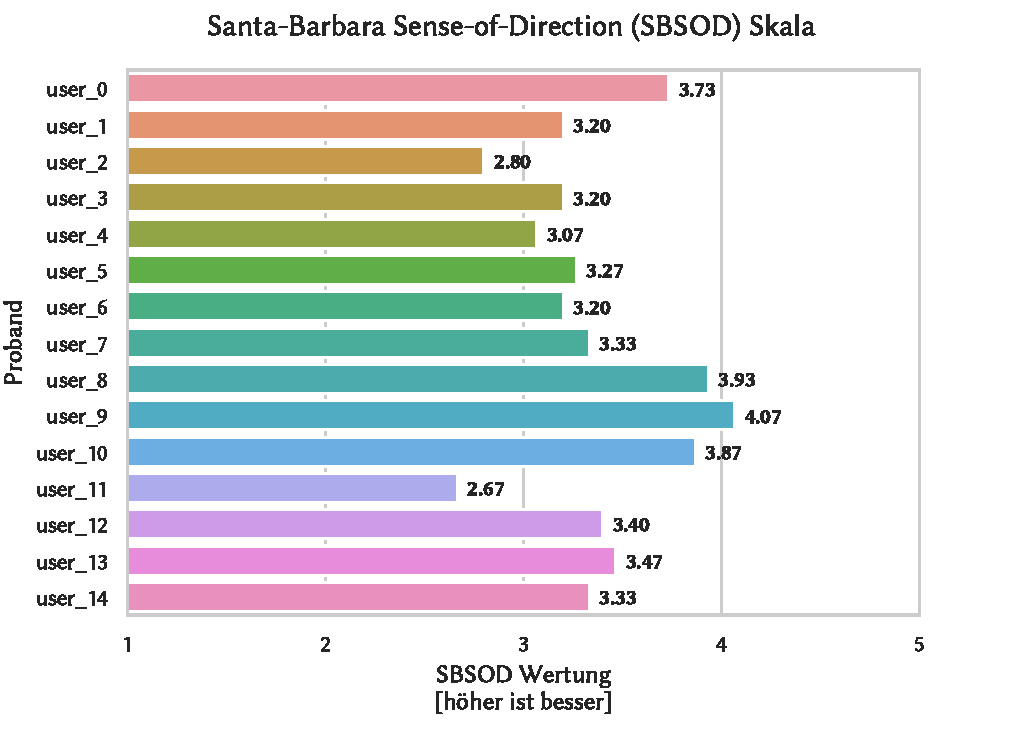
\includegraphics[trim={3cm, 0, 2.5cm, 0}, clip, width=\linewidth]{figures/analysis/sbsod}
    \caption{Erzielte SBSOD-Werte mit $\mu = \num{3,38}$ und $\sigma = \num{0,41}$.}
    \label{fig:sbsod}
\end{figure}

\subsection{Effektivität und Effizienz bei Raumsuche}
\subsubsection*{Suchzeit}
\label{ssec:searchtime}

\autoref{fig:searchtimes} zeigt die durchschnittlichen Suchzeiten bis zur Auswahl des Zielraums über alle Karten pro Kondition.
Die entsprechenden Mittelwerte und Standardabweichungen sind zur Übersicht in \autoref{tab:searchtime_overview} aufgeführt.
Zwischen den drei Konditionen ist nach dem Friedman-Test ein signifikanter Unterschied festzustellen ($\chi^2(2) = \num{63.5}, p < 0.001$).
Ein paarweiser Wilcoxon-Vorzeichen-Rang-Test zwischen den einzelnen Konditionen zeigt, dass die Suche nach dem Zielraum in $2D$ ($\SI{18.31}{\second} \pm \SI{9.3}{\second}$) signifikant schneller ist als in $3D_l$ ($\SI{27.44}{\second} \pm \SI{13.39}{\second}, z=\num{-6.003}, p<\num{0.001}$) und $3D_h$ ($\SI{28.84}{\second} \pm \SI{10.08}{\second}, z=\num{-7.136}, p<0.001$).
Der Unterschied der Suchzeit zwischen $3D_l$ und $3D_h$ ist jedoch nicht signifikant.
\begin{figure}[h]
    \centering
    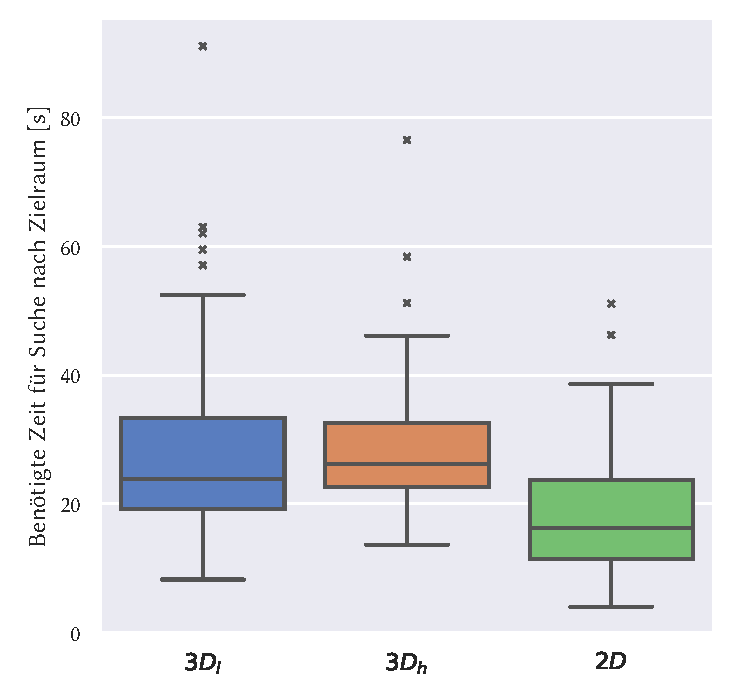
\includegraphics[width=0.7\linewidth]{figures/analysis/searchtime_boxplot}
    \caption{Boxplot der durchschnittlichen Suchzeiten (in Sekunden) über alle Karten je Kondition.}
    \label{fig:searchtimes}
\end{figure}
\begin{table}[h]
    \centering
    \caption{Mittelwert $\mu$ und Standardabweichung $\sigma$ der Suchzeit über alle Karten je Kondition.}
    \label{tab:searchtime_overview}
    \begin{tabular}{rccc}
        \toprule
        {} & \multicolumn{3}{c}{Suchzeit [\SI{}{\second}]} \\
        {} &          $3D_l$ &          $3D_h$ &          $2D$ \\
        \midrule
        $\mu$    &  $\num{27.44}$     &  $\num{28.84}$     &  $\num{18.31}$ \\
        $\sigma$ &  $\pm \num{13.39}$ &  $\pm \num{10.08}$ &   $\pm \num{9.3}$ \\
        \bottomrule
    \end{tabular}
\end{table}

Weiterhin stellt sich die Frage, ob ein \enquote{besserer} Orientierungssinn zu einer kürzeren Suchzeit führt.
\autoref{fig:correlation_time_sbsod} zeigt die durchschnittliche Suchzeit der Probanden in Bezug zu den ermittelten SBSOD-Wertungen.
Für jede Kondition wird Spearmans Rangkorrelationskoeffizient zwischen der SBSOD-Wertung und der durchschnittlichen Suchzeit ermittelt.
Die Tests weisen keinen signifikanten Zusammenhang der Variablen auf.
\begin{figure}[h]
    \centering
    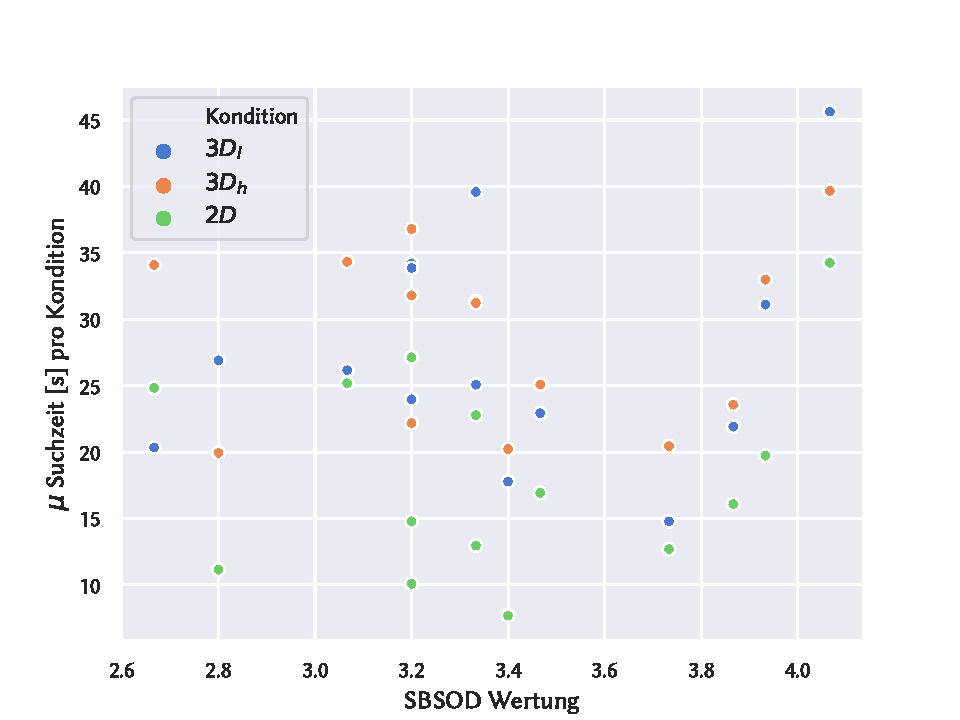
\includegraphics[width=\linewidth]{figures/analysis/correlation_time_sbsod_scatter}
    \caption{Scatterplot zur Überprüfung der Korrelation zwischen SBSOD-Wertung und Suchzeit.}
    \label{fig:correlation_time_sbsod}
\end{figure}

\subsubsection*{Fehlerrate bei Raumauswahl}
Neben der Suchzeit wurde auch die Zahl der falsch ausgewählten Räume (die Nicht-Zielräume) gemessen.
Über die insgesamt 252 Suchaufgaben (14~Probanden $\times$ 3~Konditionen $\times$ 6~Karten) wurden in drei Fällen (\SI{1,19}{\percent}) statt dem Zielraum falsche Räume ausgewählt.
\autoref{tab:error_searching} zeigt eine Übersicht der entsprechenden Events.
In beiden Fällen traten die Fehler in der ersten Kondition der entsprechenden Testsequenz ein (allerdings nicht in der ersten Karte).
\begin{table}[h]
    \centering
    \caption{Übersicht der Anzahl der falsch ausgewählten Räume während der Suchaufgabe.}
    \label{tab:error_searching}
    \begin{tabular}{rccccc}\toprule
        Proband                  & Kondition               & Karte    & Suchzeit [\SI{}{\second}] & \# Fehler & Sequenz  \\\midrule
        user\_8                  & $3D_h$                  & Karte\_6 & $\SI{40,61}{\second}$     & 2         & $3D_h$--$3D_l$--$2D$ \\
        user\_9                  & $2D$                    & Karte\_5 & $\SI{38,4}{\second}$      & 1         & $2D$--$3D_l$--$3D_h$ \\\bottomrule
    \end{tabular}
\end{table}

\subsection{Effektivität und Effizient bei Richtungsschätzung}

\subsubsection*{Genauigkeit der Schätzung}
Da in den Tests nur Layouts mit einem Stockwerk eingesetzt wurden, spiegelt die vertikale Abweichung bei der Richtungsschätzung lediglich die Fähigkeit der Probanden wieder, auf die Mitte des Laborraums zu zielen.
Folglich sind die Werte im Vergleich zur horizontalen Abweichung kleiner und unterscheiden sich kaum zwischen den Konditionen ($3D_l$: $\mu = \ang{5,74} \pm \ang{4,47}$; $3D_h$: $\mu = \ang{5,63} \pm \ang{4,06}$; $2D:$ $\mu = \ang{6,08} \pm \ang{4,8}$; absolute vertikale Abweichung).
Daher werden die Ergebnisse der vertikalen Abweichung im Folgenden nicht weiter beachtet.

\autoref{fig:horizontal_offset} zeigt das Ergebnis der Richtungsschätzung.
Da die Abweichung sowohl in positiven Winkeln (Abweichung nach rechts) als auch negativen Winkeln (Abweichung nach links) gemessen wurde, werden hier die absoluten Werte der Abweichung analysiert.
Andernfalls würden sich die Werte bei der Mittelwertbildung gegenseitig aufheben.
Wie zu erkennen ist, liegen die Mittelwerte von $3D_l$~(\ang{7,79} $\pm$ \ang{7,22}), $3D_h$~(\ang{7,84} $\pm$ \ang{7,44}) und $2D$~(\ang{6,62} $\pm$ \ang{5,28}) nahe beieinander.
Der Friedman-Test kann keine signifikanten Unterschiede zwischen den Konditionen nachweisen.
\begin{figure}[h]
    \centering
    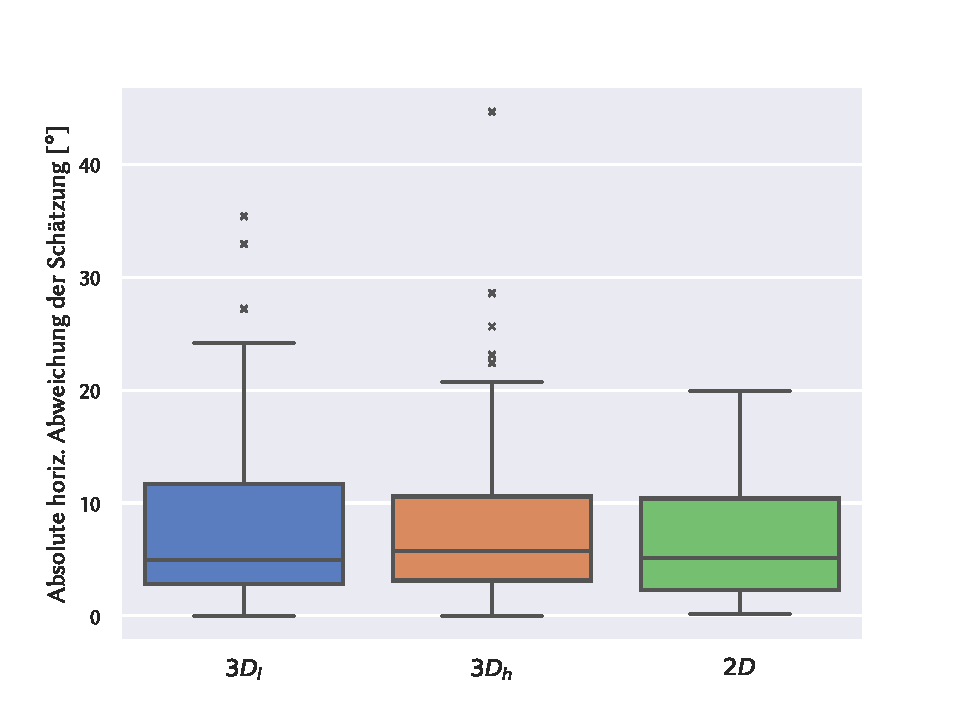
\includegraphics[height=0.45\textheight]{figures/analysis/horizontal_offset}
    \caption{Horizontale Abweichung in $\degree$ (Grad) bei der Richtungsschätzung von der tatsächlichen Linie zur Raummitte (ohne vertikale Abweichung).}
    \label{fig:horizontal_offset}
\end{figure}

Für die einzelnen Karten fasst \autoref{tab:herror_per_map} die Mittelwerte und Standardabweichungen der absoluten horizontalen Abweichungen zusammen.
\autoref{fig:horizontal_offset_per_map} zeigt den dazugehörigen Boxplot.
Es ist zu erkennen, auf Karte~3~und~4 größere Abweichungen eintreten.
Der Friedman-Test bestätigt signifikante Unterschiede zwischen den Karten ($\chi^2(6) = \num{39.755}, p < \num{0.001}$).
Die horizontale Abweichung bei Karte~3 ist signifikant größer als bei Karte~1 ($z = \num{-4,483}, p < \num{0,001}$), Karte~2 ($z = \num{-4,195}, p < \num{0,001}$), Karte~5 ($z = \num{-3,432}, p < \num{0,001}$) und Karte~6 ($z = \num{-3,37}, p < \num{0,001}$).
Auch die hohe Abweichung bei Karte~4 ist gegenüber Karte~1 ($z = \num{-3,782}, p < \num{0,001}$), Karte~2 ($z = \num{-3,395}, p < \num{0,001}$), Karte~5 ($z = \num{-2,044}, p < \num{0,05}$) und Karte~6 ($z = \num{-2,17}, p < \num{0,05}$) signifikant.
Weiterhin gibt es bei Karte~5 eine signifikant größere Abweichung als bei Karte~1 ($z = \num{-2,645}, p < \num{0,008}$), was durch die Ausreißer (siehe \autoref{fig:horizontal_offset_per_map}) begünstigt wird.
\begin{figure}[h]
    \centering
    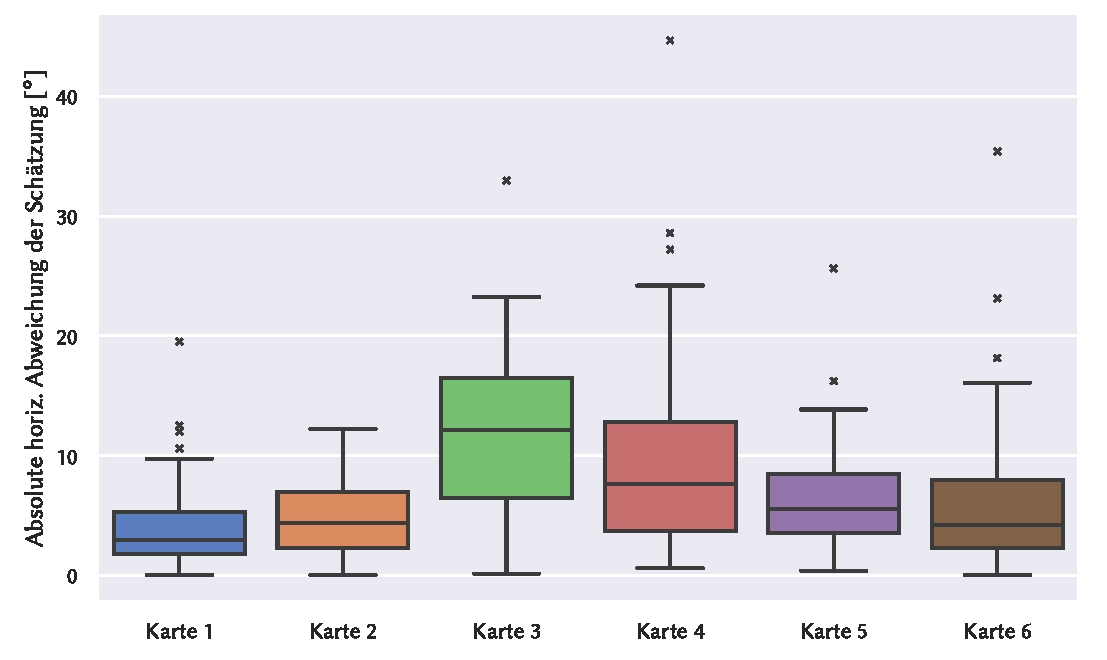
\includegraphics[width=0.75\linewidth]{figures/analysis/horizontal_offset_per_map}
    \caption{Absolute horizontale Abweichung in $\degree$ (Grad) bei der Richtungsschätzung pro Karte.}
    \label{fig:horizontal_offset_per_map}
\end{figure}%

\begin{table}[h]
    \centering
    \caption{Mittelwert $\mu$ und Standardabweichung der absoluten horizontalen Abweichung pro Karte in $\degree$.}
    \label{tab:herror_per_map}
    \begin{tabular}{cccccc}\toprule
        Karte 1 & Karte 2 & Karte 3 & Karte 4 & Karte 5 & Karte 6 \\\midrule
        $\mu = \ang{4,44}$ & $\mu = \ang{4,96}$ & $\mu = \ang{11,75}$ & $\mu = \ang{10,19}$ & $\mu = \ang{6,62}$ & $\mu = \ang{6,55}$ \\
        $\pm \ang{4,03}$ & $\pm \ang{3,3}$ & $\pm \ang{6,98}$ & $\pm \ang{9,07}$ & $\pm \ang{4,94}$ & $\pm \ang{7,05}$ \\\bottomrule
    \end{tabular}
\end{table}

Wird der Unterschied zwischen der positiven und negativen horizontalen Abweichung mit einbezogen, ist eine Tendenz zu einem Ausschlag nach links (negativ) der horizontalen Abweichungen zu erkennen.
Von den insgesamt 252~Richtungsschätzungen weichen 158 (\SI{62,7}{\percent}) nach links ab.

\subsubsection*{Schätzungszeit}
Neben der Abweichung der Schätzung wurde auch die Zeit gemessen, bis die Probanden ihr Einschätzung bestätigten.
\autoref{fig:pointing_time} visualisiert die erhobenen Daten.
In den meisten Iterationen (\SI{95,24}{\percent}) wurde die Richtungsschätzung innerhalb von 10~Sekunden bestätigt.
Im Schnitt benötigten die Probanden zur Schätzung in $3D_l$ $\SI{3,61}{\second} \pm \SI{1,71}{\second}$, in $3D_h$ \mbox{$\SI{4,18}{\second} \pm \SI{2,86}{\second}$} und in $2D$ $\SI{4,86}{\second} \pm \SI{4,78}{\second}$.
Der paarweise Vergleich weist nicht auf statistisch signifikante Unterschiede hin.
Allerdings ist eine Tendenz zu erkennen, dass die Probanden sich in der $2D$ Kondition mehr Zeit gelassen haben als in $3D_l$ ($z = -7.947,	p = 0.083$).
\begin{figure}[h]
    \centering
    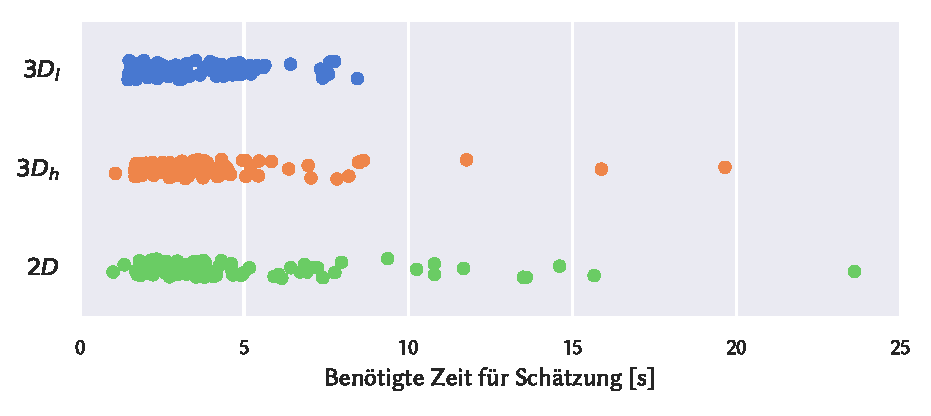
\includegraphics[width=\linewidth]{figures/analysis/pointing_time}
    \caption{Vergleich zwischen der mittleren Schätzungszeit der Konditionen, die die Probanden für die Abgabe einer Richtungsschätzung benötigten.}
    \label{fig:pointing_time}
\end{figure}

Einer der Gründe für die Messung der Schätzzeit war, die Korrelation zur resultierenden horizontalen Abweichung zu testen.
Die Überlegung ist, dass Probanden, die sich mehr Zeit für die Schätzung der Richtung nehmen, präziser sind.
\autoref{fig:pointing_time_vs_error} zeigt die absolute horizontale Abweichung in Bezug zur benötigten Schätzzeit.
Weder grafisch, noch durch Anwenden des Spearman-Tests, ist eine Korrelation zwischen den beiden Variablen erkennbar.
Da die meisten Probanden ihre Schätzung innerhalb der ersten 10~Sekunden abgegeben haben, sind für den Zeitraum \emph{nach} 10~Sekunden zu wenig Messungen vorhanden, um eine zuverlässige Aussage über eine potentielle Korrelation treffen zu können.
\begin{figure}[h]
    \centering
    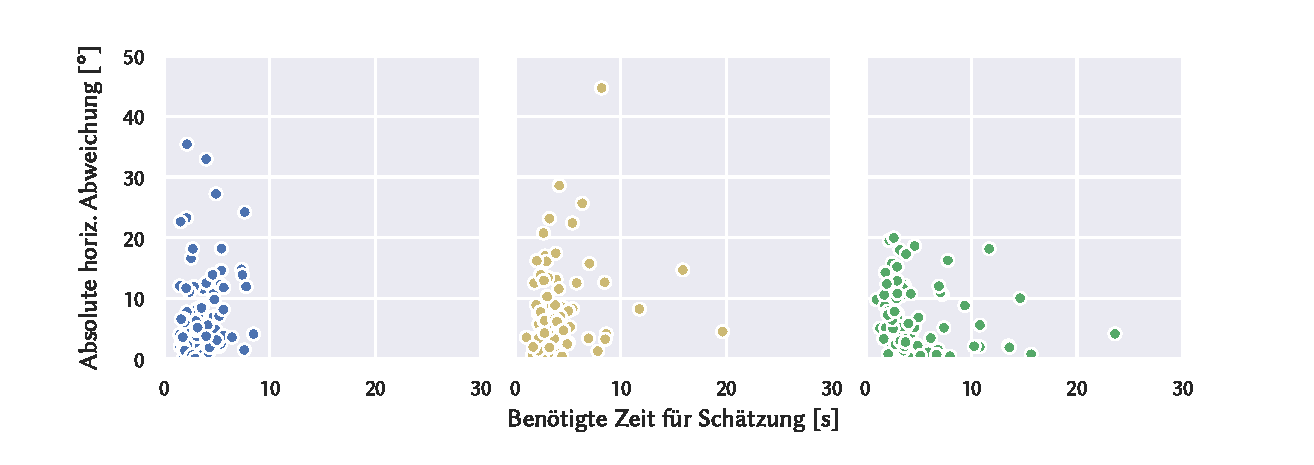
\includegraphics[width=\linewidth]{figures/analysis/pointing_time_vs_error}
    \caption{Plot der Schätzungszeit gegen die absolute horizontale Abweichung. %
    Eine Korrelation ist nicht erkennbar.}
    \label{fig:pointing_time_vs_error}
\end{figure}

\subsubsection*{Trefferrate}
Neben der Abweichung wurde auch die Trefferrate (ob der Zielraum bei der Schätzung getroffen wurde oder nicht) gemessen.
\autoref{fig:hitrate_per_user} zeigt einen Boxplot der Trefferrate über alle Probanden zwischen den einzelnen Konditionen.
Es ist anzumerken, dass für die Berechnung eines Treffers die vertikale Abweichung mit einbezogen wurde.
Die höchste durchschnittliche Trefferrate zeigten die Nutzer in $3D_h$ ($\mu = \SI{79,8}{\percent} \pm \SI{26,3}{\percent}$), gefolgt von $2D$ ($\mu = \SI{76,2}{\percent} \pm \SI{23,3}{\percent}$) und schließlich $3D_l$ ($\mu = \SI{75}{\percent} \pm \SI{20,4}{\percent}$).
Ein Friedman-Test ergab keine signifikanten Unterschiede zwischen den Konditionen.
\begin{figure}[h]
    \centering
    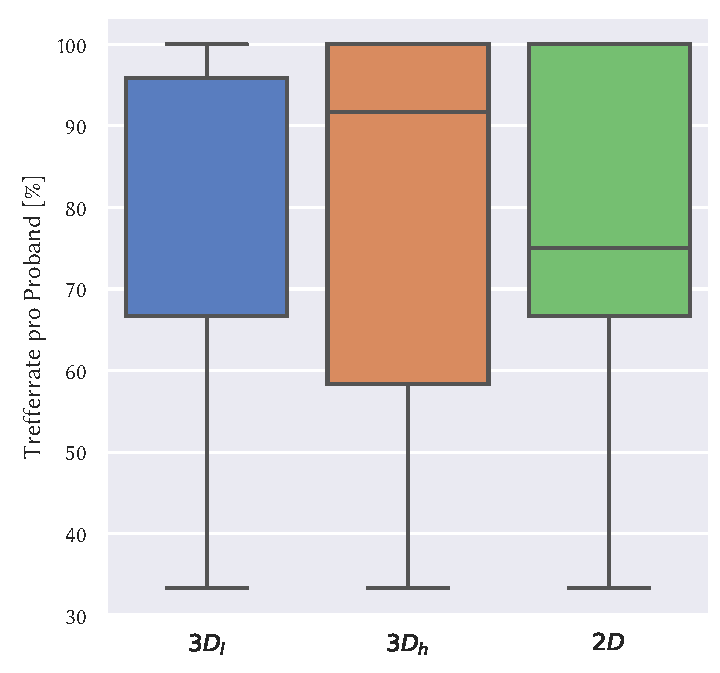
\includegraphics[width=0.7\linewidth]{figures/analysis/hitrate_per_user}
    \caption{Trefferrate des Zielraums über alle Probanden zwischen den Konditionen.}
    \label{fig:hitrate_per_user}
\end{figure}

\subsection{Fragebögen zur Nutzungsfreundlichkeit}
Die Fragebögen enthielten sowohl positiv als auch negativ formulierte Aussagen in einer ungleichmäßigen Reihenfolge, denen die Probanden auf einer Skala von 1 bis 5 zustimmen oder sie ablehnen konnten.
Für die Auswertung wurden die Bewertungen der positiven Aussagen invertiert.
Die Bewertungen wurden aufaddiert und schließlich mit einem Faktor von \num{3,125} multipliziert, um so eine Gesamtwertung zwischen 0 und 100 zu erhalten.
Es sei darauf hingewiesen, dass die Fragebögen nur acht statt, wie in der SUS vorgesehen, zehn Fragen enthalten \autocite{Brooke2013}. 
Daher sind die Wertungen der beiden Skalen nicht direkt miteinander vergleichbar.

Das Ergebnis des Fragebogens ist in \autoref{fig:usability} zusammengefasst.
Durchschnittlich bewerteten die Probanden die $2D$-Variante am besten ($\mu = \num{83,75} \pm \num{12,11}$).
Dahinter liegen die Megamaps mit $3D_l$ ($\mu = \num{72,29} \pm \num{17,27}$) und $3D_h$ ($\mu = \num{65,21} \pm \num{18.06}$).
Ein paarweiser t-Test zeigt, dass die höhere Bewertung von $2D$ gegenüber $3D_l$ ($t = 2.452, p < 0.05$) und $3D_h$ ($t = 3.988, p < 0.005$) statistisch signifikant ist.
Zwischen den beiden 3D-Konditionen gibt es keine signifikanten Unterschiede.
\begin{figure}[h]
    \centering
    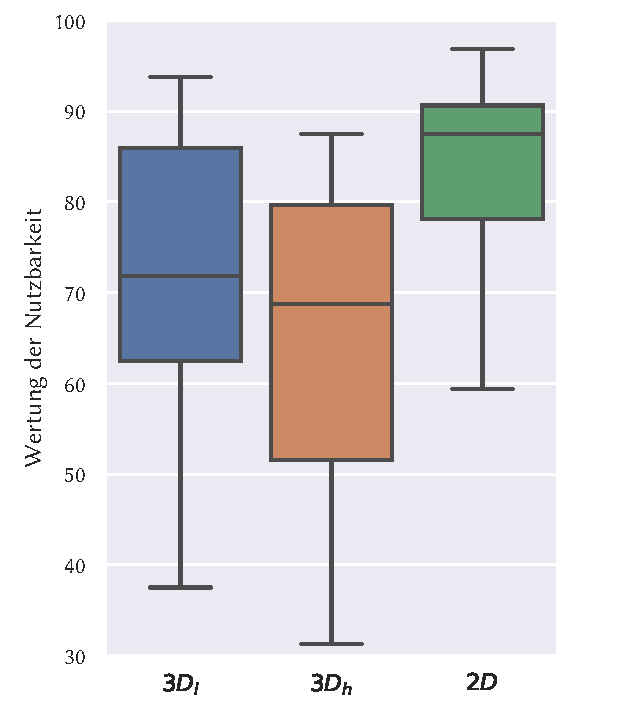
\includegraphics[width=0.7\linewidth]{figures/analysis/usability}
    \caption{Bewertung der Nutzbarkeit der einzelnen Konditionen.}
    \label{fig:usability}
\end{figure}

\section{Diskussion der Ergebnisse}

\subsection{Suchaufgabe}
Sowohl die Zeitmessungen als auch die Präferenzen der Probanden für die Suchaufgabe ist eindeutig.
Die 2D-Variante ist hier den beiden 3D-Megamaps mit einer durchschnittlichen Differenz von fast \SI{10}{\second} weit überlegen.
Es gibt drei Gründe, durch die sich dieses Ergebnis erklären lässt:

\paragraph{1.} Für die Suchaufgabe wurden die Bälle in den Räumen platziert.
Die Bälle befanden sich dabei auf Fußbodenhöhe des jeweiligen Raums.
Auf den 3D-Megamaps wurden sie dabei teilweise durch die Wände der Räume und die geöffneten Türen verdeckt.
Die Probanden mussten sich von Raum zu Raum bewegen, um in die Räume zu schauen und die Bälle sehen zu können, was zusätzliche Zeit in Anspruch nahm.
Aus den Gesprächen ergab sich, dass dieser Effekt auf der hohen Megamap zusätzlich verstärkt wurde.
$P_{14}$ meint, dass man \enquote{bei 3D [\dots] gefühlt in jeden Raum reingucken [muss].}
Die zusätzliche Höhe der Megamap vom Boden sorgte für einen flacheren Blickwinkel auf die Karte, wodurch die Räume schlechter eingesehen werden konnten als auf der niedrigen Megamap.
Einige Male wurde Bälle nicht gesehen, wodurch die Probanden die Räume mehrmals ablaufen mussten, bis sie den Zielraum entdeckten.
Auf der 2D-Karte bestand dieser Nachteil nicht, da es in der zweidimensionalen Ansicht in diesem Sinn keine Wände gibt und die Bälle nicht verdeckt werden.
Die Probanden schauten hier automatisch von oben auf die Karte und konnten so direkt in \emph{alle} Räume schauen.

\paragraph{2.}
Verbunden mit dem ersten Problem ist das unterschiedliche Sichtfeld der Karte zwischen den Konditionen.
Bei der 2D-Karte standen die Probanden mehrere Meter von der Karte entfernt und schauten \enquote{von oben} auf sie hinab.
Die 2D-Karte war somit zu jeder Zeit komplett im Blickfeld der Probanden, wodurch alle Räume und Bälle sowie der eigene Positionsmarker sichtbar waren.
Bei den 3D-Megamaps hingegen sieht das Konzept vor, dass die Probanden inmitten der Karte stehen und von ihr umgeben werden.
Das bedeutet, dass der Teil der Megamap, der sich hinter den Probanden befindet, nicht einsehbar ist.
Demnach können sich Probanden nur auf einen kleinen Teil der Karte konzentrieren.
Dies ist eine direkte Konsequenz aus der Übertragung der Megamap von der Dritte-Person-Perspektive aus TCTD in die Erste-Person-Perspektive.
Einige Probanden versuchten dieses Problem zu umgehen, indem sie sich bei jeder Karte zuerst \enquote{aus der Karte heraus} bewegten, um einen Überblick des Grundrisses zu bekommen.
$P_7$ fühlte sich von der hohen Megamap eingeengt und sagt dazu, dass er \enquote{erst einmal da rausgehen und außen herum laufen [muss].}

Ein weiteres Problem war, dass sich bei den 3D-Karten der Positionsmarker des Probanden unter Umständen außerhalb des Blickfelds befand.
Die Probanden verloren somit während der Suche den Bezug zum Laborraum.
$P_9$ beschreibt, dass sie jedes Mal nach dem Lab-Raum suchen musste, weil sie \enquote{voll auf die Bälle fixiert} war.
Der Verlust von visuellem Kontext außerhalb des Blickfelds wird z.B. in Videospielen durch die Anzeige von Markern auf Kompassleisten oder Minikarten ausgeglichen.
In der Literatur lassen sich Ansätze finden, die Gleiches für die Anwendung auf AR-VR-HMDs umsetzen \autocites{Lin2017a}{Gruenefeld2017}.
Für den konkreten Prototyp schlägt $P_3$ vor, eine visuelle Line vom Positionsmarker zur aktuellen Position des Nutzers zu ziehen.

\paragraph{3.}
Die Probanden beschrieben, dass zum Merken der Richtung für die Schätzungsaufgabe auf den Karten unterschiedliche \enquote{Taktiken} notwendig seien.
In der Tat folgten fast alle Probanden auf den 3D-Megamaps der gleichen Vorgehensweise und kehrten vor der Auswahl des Zielraums zuerst zum Laborraum auf der Karte zurück, um sich so für die Schätzungsaufgabe die Richtung merken zu können.
Ein Nutzer zielte während des Ablaufens der Karte mit dem Controller immer auf den Raum, in dem er die höchste Zahl an Bällen gezählt hatte ($P_{14}$).
Auf der 2D-Karte hingegen waren diese Taktiken nicht notwendig.
Hier orientierten sich die Probanden für das Merken der Richtung an besonderen Merkmalen auf der Karte, z.B. der Säule im Laborraum oder den Türen.
Einige der Probanden nutzen auch die Rotation des Positionsmarkers aus, um sich den Winkel für die korrekte Drehung zum Zielraum zu merken.
Z.B. bevorzugten $P_4$ und $P_6$ die 2D-Karte für die Richtungsschätzung, da diese Variante \enquote{gewohnter} sei.

Ein Aspekt, der sich (laut den Probanden) weniger auf die Performance auswirkte, als zuvor angenommen, war der Komfort der HMD-Nutzung.
Da die Probanden für die 3D-Megamaps die meiste Zeit in Richtung Boden schauen mussten, wurde der Kopf in einer geneigten Position gehalten.
Es wurde vorab vermutet, dass das Gewicht des HMDs sowie die Befestigung am Kopf für ein unangenehmes Gefühl sorgen könnte und den Eindruck, das HMD könne vom Kopf abrutschen.
In der Praxis war das nur für $P_5$.
Die anderen Probanden berichteten von keinen Problemen mit dem Komfort.
Die Tatsache, dass an den Rändern der Linse das Bild (und somit auch die Bälle in den Räumen) verschwommen war, wurde jedoch angemerkt.

\subsection{Richtungsschätzung}
Anders als bei der Zielraumsuche sind die Ergebnisse für die Richtungsschätzung nicht eindeutig.
Zwischen den drei Konditionen gibt es weder bei der Abweichung noch bei der Schätzungszeit statistisch signifikante Unterschiede.
Bei der Nachfrage im Interview nach der Präferenz für die Orientierung und Richtungsschätzung verteilten sich die Probanden zwischen $3D_l$ und $2D$.
Keiner der Probanden empfand $3D_h$ als beste Variante für die Richtungsschätzung, was mitunter auch durch die Schwierigkeiten bei der vorherigen Suche (siehe vorigen Abschnitt) einher geht. 

Auffällig ist allerdings, dass die ausreißenden Abweichungen nur in den 3D-Konditionen auftreten (siehe \autoref{fig:horizontal_offset}).
Die Aufnahme des extremsten Ausreißers ($\ang{44,68}$ auf Karte~4 in $3D_h$) zeigt, dass der Proband zuerst in die grobe Richtung des Zielraums zielt, sich dann jedoch anders entscheidet und den Controller bewusst nach rechts wegzieht.
In diesem Fall kann davon ausgegangen werden, dass der Proband sich über die gemerkte Richtung unsicher ist.
Für die anderen Ausreißer kann ein solches Verhalten nicht beobachtet werden.
Wie \autoref{fig:pointing_time_vs_error} zeigt kann auch nicht auf eine Korrelation zwischen der Schätzungszeit und dem Abweichungsfehler geschlossen werden.
Die meisten Schätzungen wurden innerhalb von 10~Sekunden abgegeben und die schnellen Einschätzungen sind nicht zwingend ungenauer als die, für die sich Probanden mehr Zeit genommen haben.
Es wird hieraus gefolgert, dass in der 2D-Karte die Orientierungspunkte (Säule, Türen, Wände, Positionsmarker) für das Merken einer Richtung besser wahrgenommen werden und somit zu weniger Unsicherheit und groben Schätzungsfehlern führen, als es bei den 3D-Karten der Fall ist.

% v.A. Unterschiede zwischen den Karten -> Besonderheit Karte 3 u. 4?
Ein Faktor, der die Höhe der Abweichung wesentlich beeinflusst, ist das jeweilige Layout der zugrundeliegenden Karte (siehe \autoref{fig:horizontal_offset_per_map}).
Bei der Gestaltung der Kartenlayouts wurde darauf geachtet, dass unterschiedliche Rotationen (vom Laborraum aus gesehen) für korrekte Einschätzungen notwendig sind.
Wie auf der Grafik zu sehen ist sind die Abweichungen in den Karten~3~und~4 am höchsten.
Die beiden Layouts sind in \autoref{fig:map_3_and_4} zu sehen.
Interessant ist, dass in diesen beiden Layouts die Zielräume \emph{fast} auf einer Geraden mit dem Laborraum liegen (\enquote{nach vorne} in Karte~4, \enquote{nach hinten} in Karte~3).
Die Mittelpunkte der Räume weichen durch einen kleinen Versatz von dieser Geraden ab.
Es wird vermutet, dass für die beiden Karten dieser kleine Versatz von den Probanden bei der Einschätzung entweder vernachlässigt oder aber als größer eingeschätzt wird, als er eigentlich ist.
Folglich entsteht für die beiden Layouts eine größere Abweichung als für die anderen Karten.
Für den Ausbau dieser Theorie bedarf es einer weiteren Studie, die sich speziell mit dem Versatz von Zielpunkten in der Umgebung im Bezug zu einem Referenzpunkt auseinandersetzt.
\begin{figure}[h]
    \begin{subfigure}{0.49\linewidth}
        \centering
        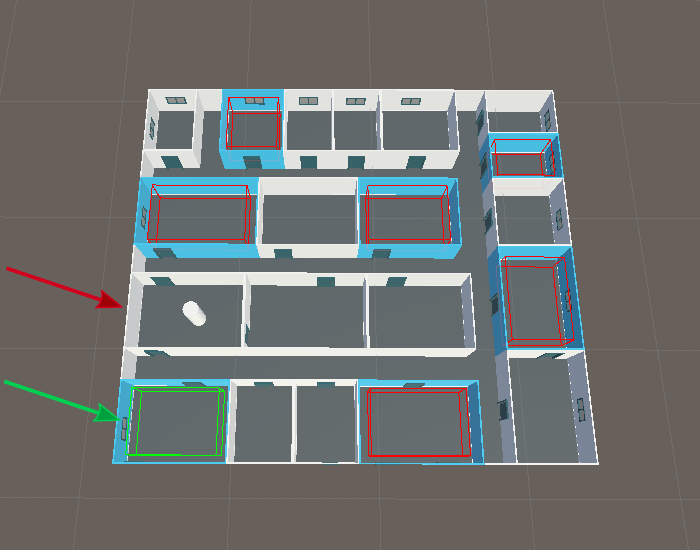
\includegraphics[width=\linewidth]{figures/screenshots/map_3_x}
        \caption{}
        \label{sfig:map_3}
    \end{subfigure}%
    \hfill
    \begin{subfigure}{0.49\linewidth}
        \centering
        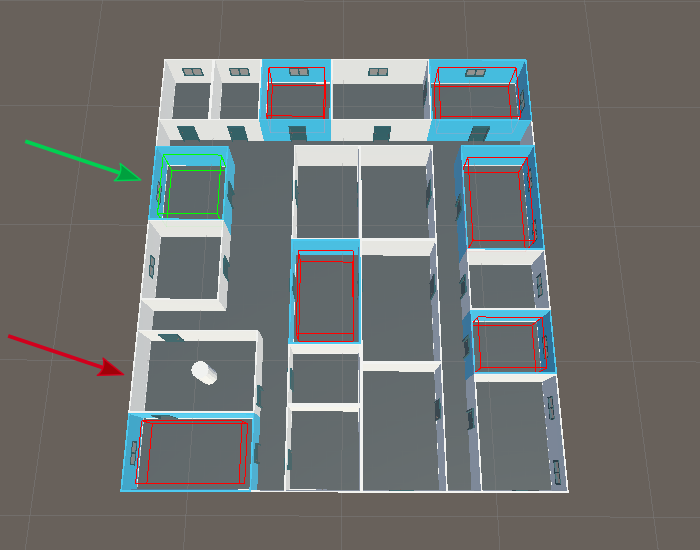
\includegraphics[width=\linewidth]{figures/screenshots/map_4_x}
        \caption{}
        \label{sfig:map_4}
    \end{subfigure}%
    \caption{Layouts der Karten 3 (\subref{sfig:map_3}) und 4 (\subref{sfig:map_4}). %
    Die blauen Räume wurden während des Tests mit Bällen gefüllt. %
    \textcolor{red}{Roter Pfeil}: Laborraum. %
    \textcolor{green}{Grüner Pfeil}: Zielraum.}
    \label{fig:map_3_and_4}
\end{figure}

Für die Schätzung wurde weiterhin eine Tendenz zu einer Abweichung \enquote{nach links} festgestellt.
Hier besteht die Vermutung, dass dies mit der Auswahl der Probanden zusammenhängt.
Von der 14 ausgewerteten Probanden waren 12 Rechtshänder.
Die beiden verbleibenden Linkshänder absolvierten den Test ebenfalls mit der rechten Hand.
Es besteht die Möglichkeit, dass dies in Kombination mit der Haltung des Vive-Controllers zu einer links-ausgerichteten Abweichung führt.
Weitere Tests mit einer ausbalancierten Zahl von Rechts- und Linkshändern sind für eine Bestätigung dieser Theorie erforderlich.

In den Interviews wurden die Probanden gefragt, ob sie sich (neben der Richtung zum Zielraum) auch die Pfade für eine potentielle Navigation zum Zielraum gemerkt hätten.
Fast alle Probanden äußerten, dass sie sich nur die groben Richtungen gemerkt hätten.
Manche der Probanden erwähnten, während der Suchaufgabe versucht zu haben, sich die Wege zu den Zielräumen einzuprägen.
$P_{13}$ hat z.B. darüber nachgedacht, durch welche Türen er zum Ziel laufen muss.

\subsection{Room-Guides und Animation}
Die Room-Guides und die Animation wurden in den Prototypen implementiert, um den Bezug des Laborraums auf der Megamap zum Laborraum in der Umgebung zu verstärken.
Die Probanden wurden hinsichtlich dieser Idee befragt.

Keiner der Probanden empfand die Room-Guides als besonders nützlich.
Manche der Probanden hatten die Linien nicht bewusst wahrgenommen.
Andere hatten die Linien gesehen, deren Zweck aber nicht verstanden.
Die Probanden äußerten, dass ihnen der Positionsmarker und die Säule sowohl im virtuellen Labor als auch auf der Karte für einen Bezug zwischen Megamap und Umgebung ausgereicht hätten.
Daraus lässt sich Schlussfolgern, dass wichtige Merkmale und Strukturen der Umgebung für eine Indoor-Karte wichtig sind, um eine schnelle Orientierung auf der Karte zu ermöglichen.

Die Animation wurde von den Probanden gemischt aufgenommen.
Ein Proband äußerte, dass die Animation \enquote{mega entscheidend} war, da er \enquote{manchmal Schwierigkeiten [habe], die [Karten] auf den echten Raum zu mappen}.
Andere Probanden empfanden die Animation jedoch als \enquote{irritierend} ($P_{14}$).
Ein Proband sagte, dass \enquote{die Animation [sich anfühlt] wie Herunterfallen} ($P_9$).
Weitere Probanden verspürten während der Animation die VR-typische Motion Sickness ($P_0$, $P_7$).
Vor allem bei der 2D-Variante war dies der Fall, da hier die Animation zusätzlich zur Skalierung auch die Rotation der Karte ändert.
Es lässt sich daraus schließen, dass die Animation, wie sie hier implementiert wurde, keine allgemeingültige Lösung für einen Bezug zur Umgebung ist und sogar kontraproduktive Effekte aufweisen kann.

\subsection{Nutzbarkeit}
Die Ergebnisse zur Nutzbarkeit der drei Varianten anhand der Fragebögen spiegeln im Grunde die Ergebnisse aus der Raumsuche wieder.
Die 2D-Karte wird von den Probanden klar bevorzugt, gefolgt von $3D_l$ und schließlich $3D_h$.
Da die Probanden die meiste Zeit des Tests mit der Raumsuche verbrachten und die Interaktionen mit den Kartenvarianten während dieses Zeitraums stattfanden, ist dieses Resultat zu erwarten.
Unter Anbetracht der Kategorisierung der SUS nach Stufen der Nutzbarkeit \autocite{Brooke2013} und der Skalierung von \num{3,125} der hier verwendeten Fragebögen erreicht die $3D_h$-Variante eine Einstufung von niedriger Nutzbarkeit.
Die Probleme der hohen Megamap wurden in den vorigen Abschnitten bereits erläutert.
Ein Vorschlag der Probanden war, die Höhe der Wände der Megamap zu verringern, sodass man bei der hohen Megamap weiterhin gut in die Räume hineinsehen kann ($P_{11}$, $P_{13}$).
Eine weitere Alternative wäre die Verwendung von visuellen Markierungen oberhalb der Räume, was dem Konzept in \autoref{chap:concept} entspricht.
Hier bestünde keine Notwendigkeit, in die Räume hineinzusehen.

Besonders positiv wurden die Megamap-Varianten bezüglich ihrer Eignung zur Orientierung (\enquote{Wo bin ich?}) bewertet.
Dies unterstützt die Vermutung, dass sich durch die Megamaps ein räumliches Verständnis von der eigenen Umgebung aufbauen kann.

\subsection{Zusammenfassung}
Der Prototyp wurde in dieser Arbeit entwickelt, um mit der Nutzerstudie zwei Fragen zu klären:
Erstens, ob sich mit einer dreidimensionalen Megamap ein räumliches Verständnis von der Umgebung des Nutzers aufbauen kann.
Zweitens, ob die Effektivität und Effizienz der Megamap mit einer herkömmlichen 2D-Darstellung vergleichbar ist.

Die Studie zeigt, dass durch die Verwendung der Megamap in der Tat ein räumliches Verständnis der Indoor-Umgebung des Nutzers vorhanden ist.
Nutzer können mit der Karte aus einer Reihe von Räumen unter festgelegten Suchkriterien einen Zielraum finden und sich die Richtung zu diesem Raum merken.
Außerhalb der Kartenansicht bleibt die Vorstellung, wo sich dieser Raum in der Umgebung befindet, erhalten.
Wie $P_3$ und $P_7$ richtig erkennen, gehört für eine explorative Kartenanwendung mehr dazu, als ein simples räumliches Verständnis von Richtungen.
Erst durch die Einbindung einer Suchfunktion für Objekte und die Integration von Informationen über die Umgebung kann eine Megamap als Kartenanwendung verwendet werden.
Der vorliegende Prototyp setzt viele der Aspekte aus \autoref{chap:concept} nicht um, weshalb er nur als sehr limitierte Variante einer Megamap bezeichnet werden kann.
Der eigentliche Mehrwert der Megamap entsteht erst durch die \emph{inhaltliche} Integration in die Umgebung und umgekehrt.
Dieser erste Prototyp wird zwar \enquote{physisch} in die Umgebung integriert, eine inhaltliche Verbindung zur Umgebung gibt es allerdings nicht.

Die Nullhypothese dieses Experiments, dass es keinen signifikant messbaren Unterschied in Effektivität, Effizient und Nutzbarkeit zwischen einer 2D-Darstellung und den 3D-Megamaps gibt, wird \emph{teilweise} abgelehnt.
In der Suche nach Objekten auf der Karte ist die 2D-Darstellung signifikant schneller als die verglichenen Megamap-Varianten.
Ebenso (und deswegen) erhielt die 2D-Darstellung eine statistisch signifikant höhere Bewertung der Nutzbarkeit von den Probanden.
Bei der Effektivität (Trefferrate und Abweichung beim Zeigen in Richtung Zielraum) bestehen keine signifikanten Unterschiede zwischen den Konditionen.
Die Studie bestätigt damit die Ergebnisse aus \autocite{Chittaro2006} und teilweise \autocite{Li2013}, bei denen ebenfalls 2D- gegen 3D-Darstellungen von Indoor-Karten getestet wurden.
Für diese Arbeit wurde eine wesentliche Verbesserung der Effektivität der 3D-Karte erhofft, ermöglicht durch die Verwendung eines HMDs und die direkte Integration der Karte in die Umgebung.
Dieser Effekt blieb jedoch aus.

%
\cleardoublepage
